\section{Results}

\subsection{Single-shot model performance}
\label{subsection:single-shot}
% How did we come up with linear models:
% 	- compare performance of all models by "recall"
% 	- compare time with the actual docking time
% 	- test effects of normalization

% In order to select most promising models for active-learning iterations, we first compared them on a single batch (figure \ref{fig:fig_4}). 

First, it's clear that tested models have different performance on different datasets assessed in this study. Namely, for datasets where the scores were obtained with DOCK (D4 and AmpC), recall scores tends to be higher than for those obtained with ICM.

Second, it's clear that the increase in the training dataset size does not lead to significant improvements in the models performance, in line with previously observed results \cite{Yang2021_shoichet_active_learning}. Despite that, "heavyweight" model such as RandomForestRegressor, seem to benefit by that more, compared to more "lightweight" linear models, which seem to saturate at train size around $160\ 000$.

Linear models also show more stable performance across the datasets: namely, default LinearRegression and LinearSVR show recall score similar to that of RandomForestRegressor on all datasets except for CB2, where LinearRegression shows twice smaller recall values compared to LinearSVR and RandomForestRegressor. Intestingly, adding regularization to linear models does not increase their performance, as seen by LassoCV and RidgeCV performance.

\subsection{Extrapolation of single-shot results}
Following the robust performance of LinearRegression in single-shot regime, we compared its active learning regime with its extrapolation from a single-shot performance (Figure TODO). First, the results clearly show that for the large batch size (6 and 12 iterations TODO \textit{put batch size here}), extrapolation cal reliably predict the outcome of the memory-less active learning. However, with the decrease of the batch size, the extrapolation seems to be overestimating the performance (24 and 30 iterations TODO \textit{put batch size here}). Despite that, the superior performance of active learning with smaller batch size is still clear (also see Table TODO). 

It is worth noticing that results go in line with the previous results (Graff et al. \cite{Graff2021AcceleratingLearning}, Figure 5): if we look at the absolute numbers of molecules explored, we can see that the percentage of top-1000 molecules found increases with the increase in the step size. We find that the absolute number of ligands docked, and not the number of active learning steps, is more reasonable scale in this case, since the docking itself is, in our case, the most time-consuming step.

Interestingly, when using second docking run as a docking score predictor, it shows superior performance in the first few iterations, but than its predictions yield less real hits per step than the random search (Fig XX, datasets AA2AR and CB2). This is likely due to the fact that the VSHs are quickly exhausted at the first few steps, and the second docking reliability is much lower for ligands with lower scores. Potentially, comparing number of VSHs in the real active learning run with the number of VSHs from a random choice, might serve as a stopping criteria for the screening campaign.

\subsection{Optimal parameters of the active learning regime}
The meta-parameters of the active regime focused on adding memory of the docking results between different batches, as well as increasing the training size between batches. Here we discuss the \textit{early} recall (percentage of VSHs obtained after docking approx. 10\% of the library) and \textit{late} recall (after docking 30\% of the library).

Different datasets have drastically different model performance: while for AmpC dataset, around 90\% of the VSHs are found already after screening the first 10\%, for the CB2 dataset even the best late recall is around 80\%, also requiring three times as much ligands docked. Besides, the relative model performances between different datasets are more clear.

For different meta-parameters the decrease of the training size is also beneficial here (Table YY TODO: \textit{add the actual table}), in agreement to the memory-less regime and the extrapolation of single-shot results. For different datasets, the smallest vs. largets batch size (num. of iterations 6 vs num. of iterations 30 TODO: \textit{add batch size instead of number of iterations}) results 2-3 times difference in the early recall, although difference in late recall is less significant.

Adding simple model ensembling via either MeanRank or TopFromEveryModel mechanism, or simply increasing train size (LastModel with "add" parameter) confidently boosts performance: both early and late recall is 10-15 percent points higher for all the models with a memory mechanism.

However, differences in model performance with different memory mechanisms is less obvious. If we focus on the "noadd" regime, that keeps the training size constant between the batches, we can see that at 30 iterations (TODO: \textit{change to batch size}) ensembling regime MeanRank has better performance compared to two other methods. In this regime, each base model learns a piece of valuable information about its chemical subspace, and low-ranked molecules from a single base model still can end up in the final list of hits for the next iteration.

Interestingly, gradually increasing the train size does not boost the overall performance of the active learning regime. While it does increase performance for the LastModel ensembling, adding memory to the model, it does not increase the overall performance of other models, implicitly having memory mechanisms. It agrees well with the single-shot performance results and the choice of simple LinearRegression models, that seem to saturate in their performance at around $16\ 000$ batch size.

Also, even though the memory-less LastModel regime shows worse performance compared to others, it its still considerably higher than the performance of the random choice screening. For example, for the least performative CB2 dataset, it still finds around 34\% of the VSHs after screening only 10\% of ligands, around half of the VSHs for D4 and AA2AR datasets, and 86\% VSHs for the AmpC dataset.


% First, we selected diverse regression models (figure \ref{fig:fig_4}, first row), and compared them with lower-bond and upper-bond baselines. Namely, we trained the regression models to predict the docking score directly, then selected top-1\% from the sorted list as model's hits, and compared model's hits with actual top-1\% of the list. Lower-bond baselines included sklearn's DummyRegressor, as well as custom models yielding random score from either normal or uniform distribution, matching original distribution of scores (RandomUniform and RandomGaussian regressors, respectively). For upper-bond baseline, we used docking scores, provided by the second run of Molsoft's ICM (figure \ref{fig:fig_1}) without fixing a seed value.

% From this run, it is clear that linear regression performs at the level of more sophisticated models. Thus, we selected these models to test on dataset of 5zty docking scores. Surprisingly, linear regression itself showed baseline performance, while it's weighted versions, such as Lasso and Ridge regression, performed at the level with more sophisticated models.

% Last, we tested both sophisticated regression models and linear models, on known datasets obtained with DOCK \cite{ultralarge_docking_first}. As expected, different models show comparable recall, that also becomes more reproducible with the increase of the train size dataset. More complex models such as RandomForestRegressor show superior performance compared to more simple models. 

% Single-batch models share multiple trends for all models and train sizes. First, all models outperform the random baselines, as expected. Surprisingly, linear models with and without regularization don't differ by their performance. For more complicated models such as random forest and decision tree regressors, an increase in prediction quality with increase of model training size. 

% Paragraph about effect of normalization

\begin{figure}[h]
% Fig 4: selection of the best single model
% 	- A: model performances
% 	- B: model timing
% 	- C: time vs performance distribution + actual docking time cutoff
\centering
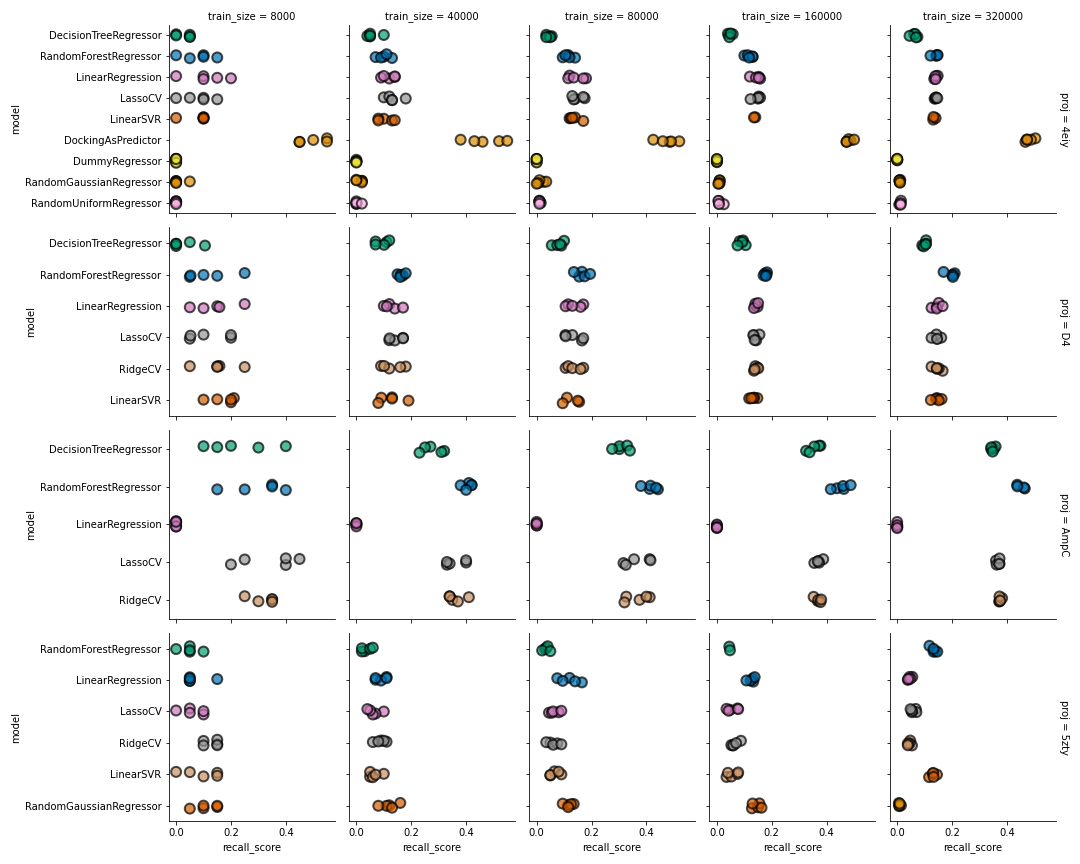
\includegraphics[width=0.8\textwidth]{figures/Figure_4.png}
\caption{Model performance for multiple regression models and their baselines on 4 datasets present in the study. \texttt{recall\_score} shows the share of interception of top-1\% of the regressor's predictions with the actual top-1\%, sorted by docking score}
\label{fig:fig_4}
\end{figure}


% To optimize meta-parameters of the active learning regime, we selected LinearRegression as the "base" learner. The choice was based on it's superior speed (see fig. TODO) and performance comparable with more complex models (figure \ref{fig:fig_3}). Active learning models were compared by their ability to retrieve top-1\% hits from the \texttt{4eiy} dataset, and compared with upper-and lower-bond baselines, as described in \ref{subsection:single-shot}. Each model had a fixed batch per single iteration, so that exactly \texttt{train\_size} scores were added to the training data on each iteration. Also, we tested the effect of the increasing (\texttt{add\_to\_train=True}) or constant (\texttt{add\_to\_train=False}) training dataset size, with the latter presumably providing the ability for the model to escape local minima in the chemical space. Finally, we tested the selection regime for the next batch: with \texttt{LastModel}, only the model from the previous batch was taken into account; with \texttt{MeanRank}, the mean molecule rank among models on all iterations was used as its score; and with \texttt{TopFromEveryModel}, all models from all iterations contributed equal amount of molecules to the next batch.


% How did we come up with iterations scheme:
% 	- compared different train sizes
% 	- compared different regimes (add/noadd)
% 	- compared different ensembling methods
% 	- compare with "docking-as-predictor"

% \begin{figure}[h]
% Fig 5: fine-tuning metaparameters of "iterations" 
% 	- batch size effect on the iterations performance
% 	- add/noadd & different ranking schemes effect
% 	- comparison  of the best model with with docking-as-predictor
% 	- TODO: comparison with the really best single model
% \centering
% 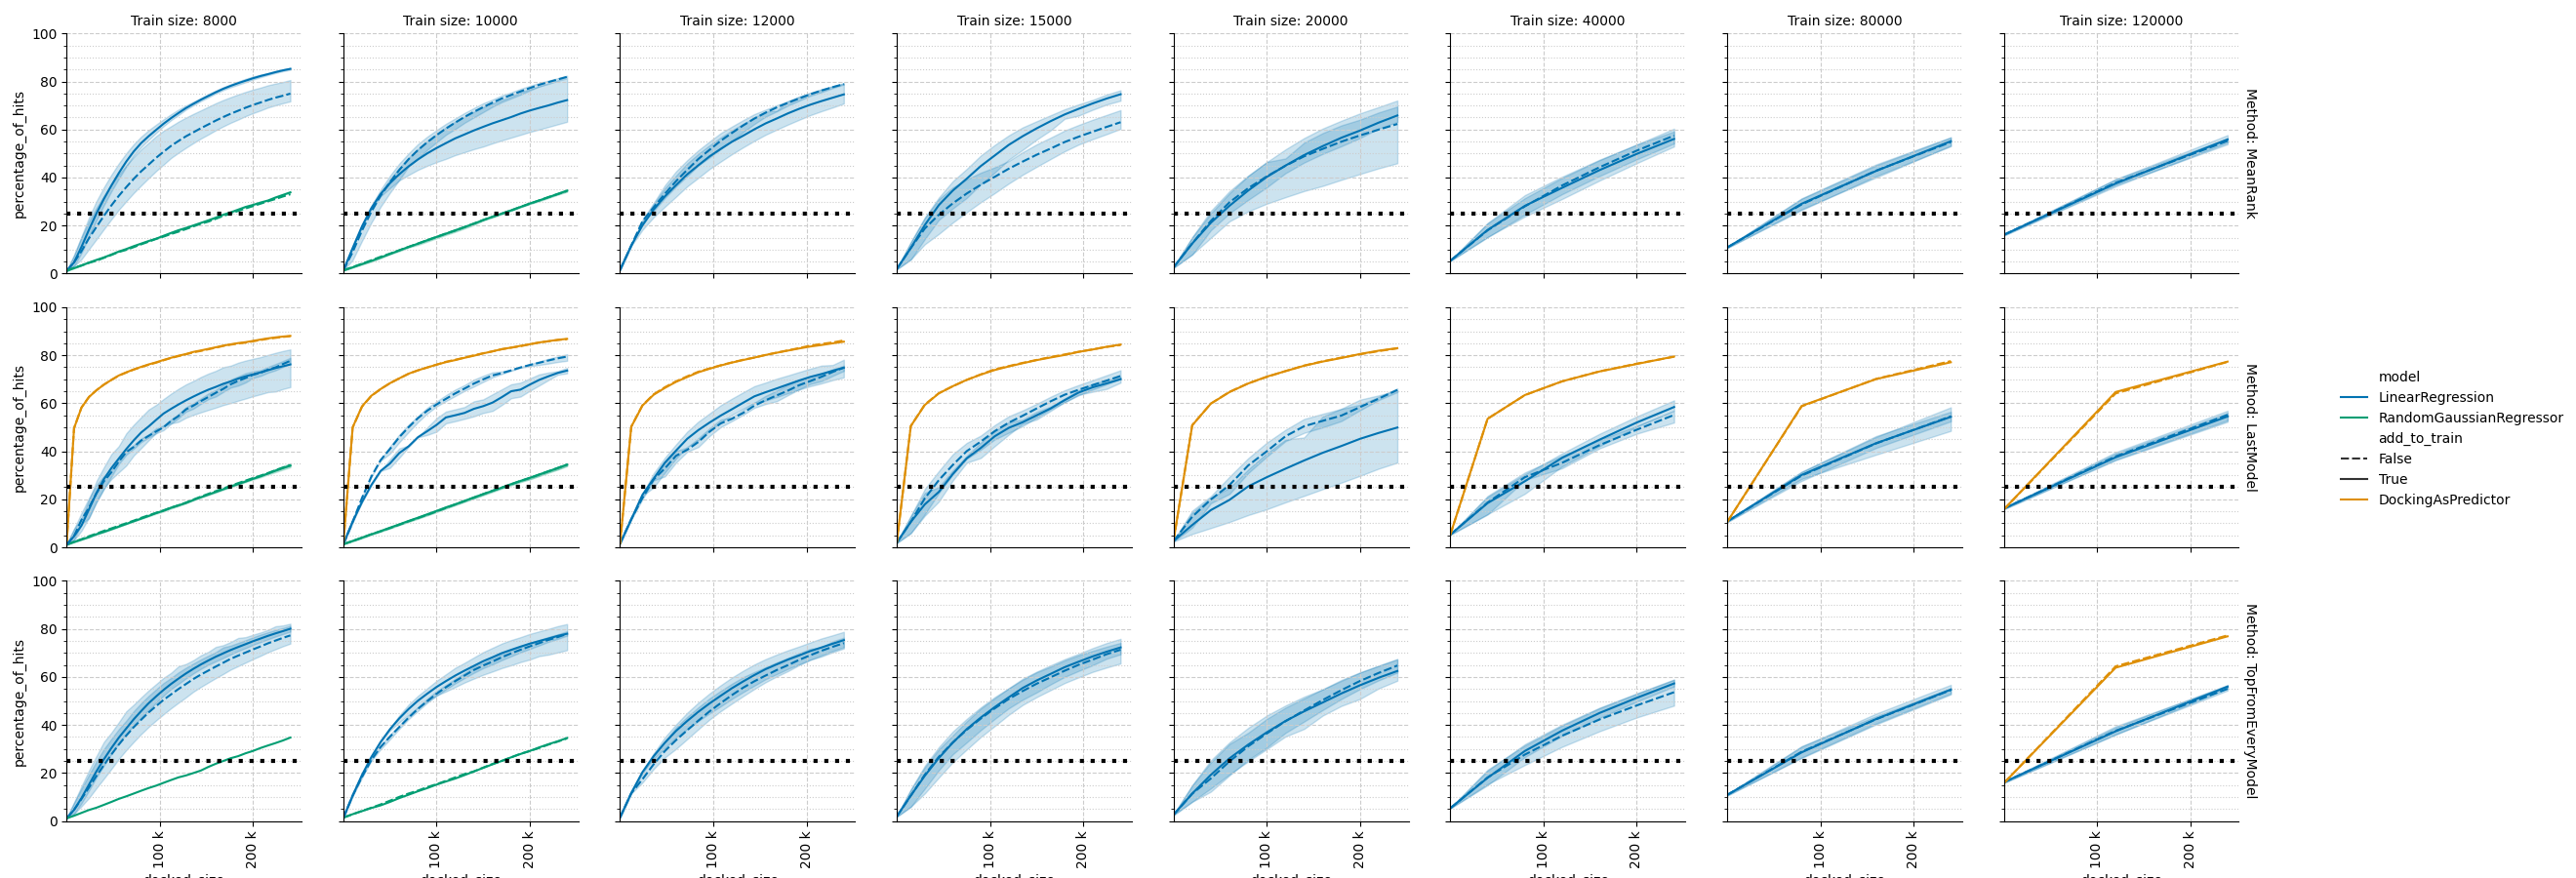
\includegraphics[width=0.8\textwidth]{figures/Figure_3_4eiy.png}
% \caption{Model performance in active learning regime}
% \label{fig:fig_3}
% \end{figure}

% Interestingly, the \texttt{train\_size} effect for the active learning regime was different from the single-batch mode. Namely, smaller training size resulted in better model performance regardless of other active learning meta parameters (figure \ref{fig:fig_3}). Smallest training size of $8~000$ resulted in retrieval of $\approx80\%$ of top-1\% molecules, while largest training size of $120~000$ resulted in mere $\approx60\%$, even though mean recall for a single-batch regime is $0.11(7)$ and $0.15(1)$, respectively. Besides, neither the next batch selection regime nor the \texttt{add\_to\_train} parameter do not have an influence within the observed data.


% Paragraph about comparison with upper- and lower-bonds.

% Paragraph about comparison of upper-bond between selection regime (probably one selection  regime is just better than the other one, if we have "ideal" data).


% \begin{figure}[h]
% \centering
% 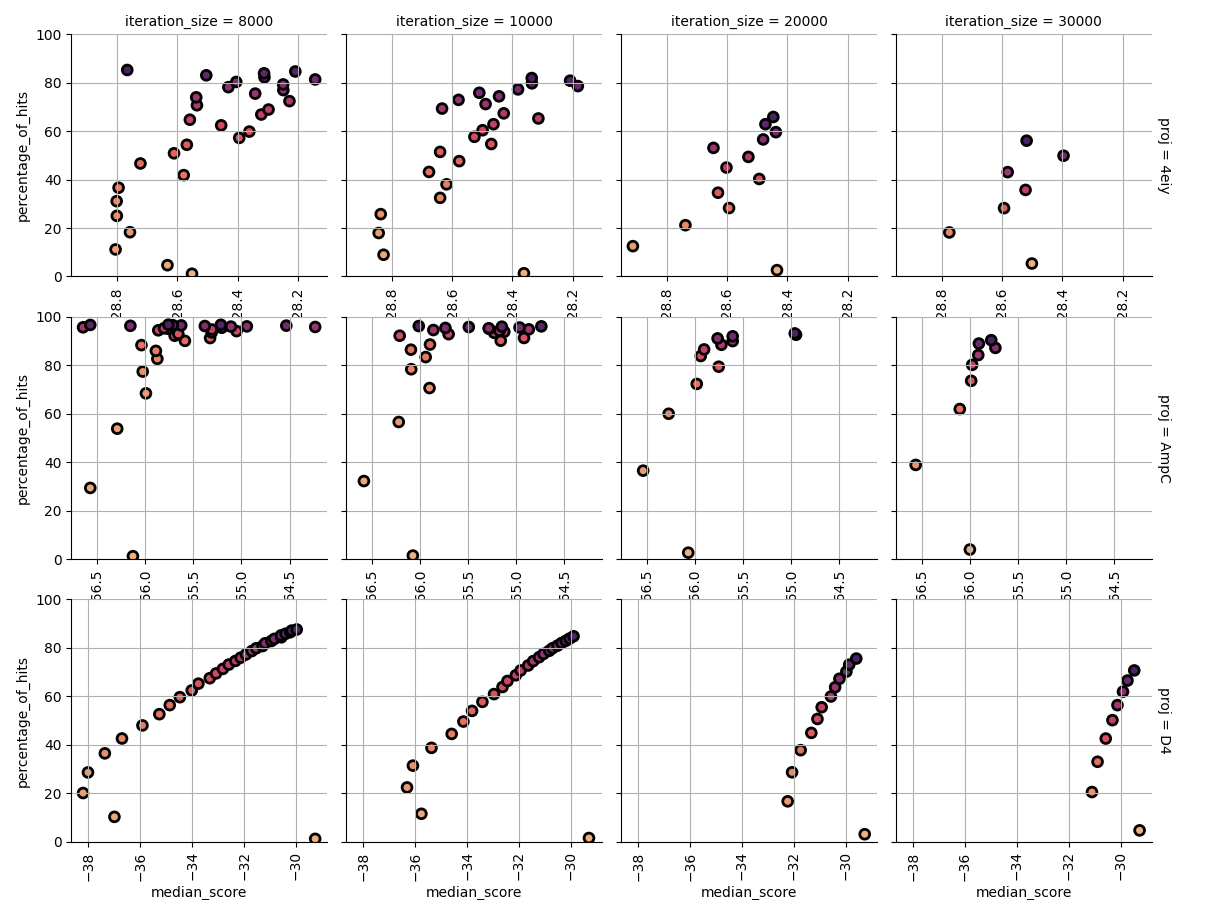
\includegraphics[width=0.8\textwidth]{figures/Figure_3_dockscore.png}
% \caption{Model performance in active learning regime}
% \label{fig:percentage_vs_dockscore}
% \end{figure}
